\documentclass[twoside,12pt,a4paper,titlepage]{article}

\usepackage{xspace}
\usepackage{siunitx}
\usepackage{booktabs}
\usepackage{rotating}
\usepackage[margin=2.5cm]{geometry}

\newcommand{\org}{SourceBots\xspace}
\newcommand{\staff}{SourceBots staff\xspace}
\newcommand{\gamename}{Pirate Islands\xspace}
\newcommand{\timeline}{April 2018\xspace}

\title{\gamename}
\author{\org}
\date{\timeline}

\usepackage{helvet}
\renewcommand{\familydefault}{\sfdefault}

\usepackage[pdftex]{hyperref}
\hypersetup{
    linkcolor=magenta,
    colorlinks=true,
}

\newcommand{\figref}[1]{
    \hyperref[#1]{Figure~\ref*{#1}}%
}
\newcommand{\regref}[1]{
    \hyperref[#1]{Regulation~\ref*{#1}}%
}
\newcommand{\ruleref}[1]{
    \hyperref[#1]{Rule~\ref*{#1}}%
}
\newcommand{\specref}[1]{
    \hyperref[#1]{Specification~\ref*{#1}}%
}
\newcommand{\subspecref}[2]{
    \hyperref[#2]{Specification~\ref*{#1}.\ref*{#2}}%
}

\begin{document}

\begin{titlepage}
\begin{center}
\textsc{\large SourceBots 2018}\\[3.5cm]
\begin{figure}
    \centering
    
\includegraphics[scale=1]{fig-sourcebots.pdf}
\end{figure}
\textsc{\huge \textbf{\gamename{}: Rules}}\\[1cm]
\textsc{\large \timeline}\\[3cm]
\end{center}
\end{titlepage}

\section{Game Rules}
\label{sec:rules}

\begin{enumerate}
  \item The game, called \emph{\gamename}, is played in the arena defined in
        \specref{spec:arena}. The objective is to collect tokens, and to bring
        them to one's scoring zone in addition to removing opponents tokens from
        your zone.
  \item The arena contains 20 tokens. The layout is detailed in
        \specref{spec:arena}. Each token of a matching colour placed in your
        zone is worth 3 points. Each token of a non-matching colour placed in
        your zone is worth -1 points: that is, a non-matching colour will lose
        points.
  \item At the end of the game, each robot is awarded the sum of the value of
        all tokens within their scoring zone (see rule \ruleref{rules:token})
  \item An additional 1 bonus point is awarded if a robot moves out of its
        starting zone.
  \item \label{rules:token}A token is in a scoring zone if, and only if, it
        has three corners in contact with the floor in the zone.
  \item Participating teams must present their robots to match officials at
        least one minute before the start of each match.
  \item There will be up to 4 robots in each match.
  \item \org may have any number of match officials within the arena, including
        during the course of matches.
  \item At the start of each match, robots must be entirely within their
        starting zones.
  \item At the start of each match, teams will be permitted to lean into the
        arena and start their robots.
  \item Each match lasts $150$ seconds.
  \item During matches teams must not touch or interfere with any part of the
        inside of the arena (including robots and tokens), except to start their
        robot under the direction of match officials.
  \item Teams may be disqualified from one or all matches by match officials,
        for non-compliance with regulations, lateness to the match, or any other
        reason at the discretion of the judge. Teams disqualified before the
        start time of a match will not be permitted to enter a robot.
\end{enumerate}

\clearpage
\section{Regulations}
\label{sec:regs}

\begin{enumerate}
\item The Judge's decision is final.
\item All robots must be safe.
  \begin{enumerate}
    \item This is defined considering safety concerns including, but not limited
          to:
      \begin{enumerate}
        \item sharp edges;
        \item the effects of impact at speed;
        \item fire risks from the battery (see Rule~\ref{rule:lipo}).
      \end{enumerate}
    \item No robots will be permitted to compete without passing a safety and
          compliance inspection.
    \item \org may reinspect your robot and invalidate previous inspections at
          any time.
  \end{enumerate}
\item Any assistance from \org staff and volunteers is provided without
      guarantees.
\item Competitors are expected to behave within the spirit of good
      sportsmanship.
\item Competitors must take reasonable measures to avoid their robot damaging
      the arena, or anything within it, including other robots. This is a
      non-contact sport.
\item All robots must be fully autonomous once started. No remote control
      systems are permitted.
\item At the start of each match, all competing robots must fit within a cube
      with edges of length \SI{500}{mm}. Expansion beyond this limit during the
      course of a match is permitted.
\item \label{rule:lipo}
      The Lithium-Polymer battery is the most dangerous part of a \org
      electronics kit and must be treated accordingly. Whenever a robot is in
      operation its battery must be:
  \begin{enumerate}
    \item securely held in place;
    \item adequately protected from damage even in the presence of damage to the
          rest of the robot;
    \item connected only to the main input of the power board.
  \end{enumerate}
%\item Additional batteries or other energy storage must be explicitly and
%      individually approved by \org before use.
\item A robot's main power switch must be easily accessible and on the top of
      the robot whenever the robot is powered.
%\item All robots must have badge mountings as described in
%      Specification~\ref{spec:badges}.
\item All electronics on a robot must be:
  \begin{enumerate}
    \item securely held in place;
    \item easily removable.
  \end{enumerate}
\end{enumerate}


\clearpage
\section{Specifications}
\label{sec:specs}
\newcounter{SpecID}

\subsection{Markers}
\refstepcounter{SpecID}
\label{spec:markers}

The arena and tokens in the game are labelled with fiducial
markers. Each marker number is associated with a particular feature in the
arena, and also has an associated size. The marker numbers and sizes are as
follows:

\begin{center}
\begin{tabular}{lcc}
  \toprule
  \textbf{Item} & \textbf{Marker Number} & \textbf{Marker Size (\si{mm})} \\
  \midrule
  Arena boundary & 0 -- 27 & 250 \\
  Columns & 28 -- 43 & 250 \\
  Tokens belonging to the robot in zone 0 & 44 -- 48 & 100 \\
  Tokens belonging to the robot in zone 1 & 49 -- 53 & 100 \\
  Tokens belonging to the robot in zone 2 & 54 -- 58 & 100 \\
  Tokens belonging to the robot in zone 3 & 59 -- 63 & 100 \\
  % Robot Badges & 69 -- 73 & 100 \\
  \bottomrule
\end{tabular}
\end{center}

All markers are oriented vertically such that the human-readable text
is under the marker.

\subsection{Arena}
\refstepcounter{SpecID}
\label{spec:arena}

\begin{enumerate}
  \item The arena floor is an \SI{8}{m} $\times$ \SI{8}{m} square. The tolerance
        of these two dimensions is $\pm$\SI{250}{mm}.
  \item The floor of the arena is carpeted.
  \item The layout of the arena is given in \figref{fig:arena}.
  \item The outer walls of the arena are at least \SI{600}{mm} high, and the
        interior surface is white plastic-coated hardboard.
  \item Each wall of the arena features seven \SI{250}{mm} fiducial markers.
        The positions of these markers is given in \figref{fig:sidewall}.
        The marker numbering is given in \figref{fig:arena}.
  \item The robot starting zones are squares which share corners with the arena
        itself. Their sides are of length \si{1}{m}.
  \item Starting zones are numbered 0,1,2,3 clockwise starting at the north west corner.
  \item In the arena there are 4 fixed square columns with a height greater than
        or equal to \SI{370}{mm}, and a width of \SI{370}{mm}.
  \item Columns will have 4 different markers on each face, as given in
        \figref{fig:arena}.
  \item Markers will be placed on columns such that there is a \SI{120}{mm} 
        gap at the bottom.
  \item The scoring zones are squares of sides \si{2815}{mm}$\pm$\SI{50}{mm}
        positioned with the columns separating them.
  \item The starting and scoring zones is visually delineated on the floor of
        the arena by coloured tape. The outer edge of the tape indicates the
        outer edge of the zone. This tape is for visual reference only.
  \item \label{spec:tokenpos} Tokens will be placed in undisclosed layouts
        within an inner \si{2}{m} square of each scoring zone. The inner square
        is positioned such that two of its edges are the inside edges of the
        scoring zones. Tokens will start at least \si{150}{mm} from columns
        or other tokens and their layouts will be rotationally symmetric to
        that of other zones.
  \item Tokens will be placed in the scoring zone on the opposite side to their
        matching coloured scoring zone.
  \item \label{spec:flags} Flags will be cylinders with a diameter
        of \si{15}{mm}, and a length of \si{200}{mm} or longer. There will be
        a decoration attached \si{100}{mm} from the top, with a height of \si{100}{mm}
        and a width of \si{150}{mm}, as described in \figref{fig:flag}. The
        cloth part of the flag must be visible when attached to the mount.

\end{enumerate}

\begin{sidewaysfigure}
  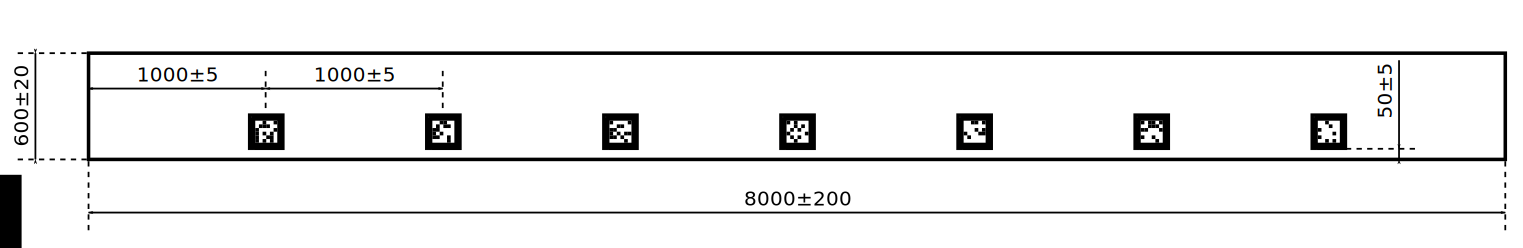
\includegraphics[scale=0.58]{fig-sidewall.pdf}
  \caption{Layout of markers along each arena wall.}
  \label{fig:sidewall}
\end{sidewaysfigure}

\begin{figure}
  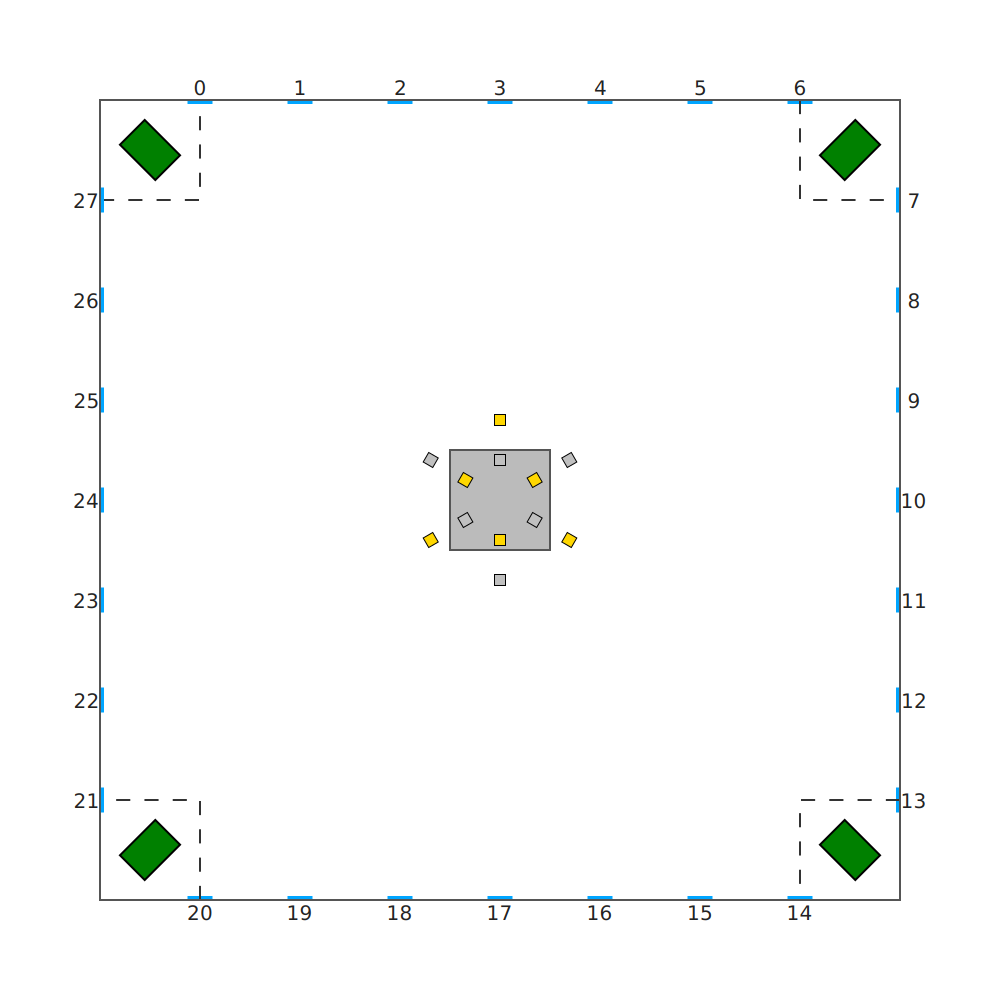
\includegraphics[scale=0.58]{fig-arena.pdf}
  \caption{Layout zones and tokens in the arena. Please note that tokens will
  be placed randomly but rotationally symmetrically within the respective
  scoring zones.}
  \label{fig:arena}
\end{figure}

\begin{figure}
  
\includegraphics[scale=0.3]{fig-flag.pdf}
  \caption{Specification of a robot flag}
  \label{fig:flag}
\end{figure}
\subsection{Tokens}
\refstepcounter{SpecID}
\label{spec:tokens}

\begin{enumerate}
  \item Tokens are cubic corrugated cardboard boxes, with sides of length
        \si{110}{mm}$\pm$\si{10}{mm}.
  \item Tokens will be coloured to match the colour of a scoring zone.
  \item Each face of each token has a fiducial marker attached.
  \item The initial layout of tokens in the arena is defined in
        \subspecref{spec:arena}{spec:tokenpos}.
\end{enumerate}

\clearpage

\section{Change Log}

Since first publication, this document has had the following changes made:

\begin{itemize}
    \item 11\textsuperscript{th} April 2018:
    \begin{itemize}
        \item The specified size of the scoring zones are now slightly smaller,
              to allow for the pillars to be between the zones without overlap.
              The diagram of this was already correct and is unchanged.
        \item The marker numbers used on tokens have been changed so that each
              robot has a consistent number of markers. The API and example
              markers in the docs were already correct and have not changed.
    \end{itemize}
\end{itemize}

\end{document}
